\scanpage{91}

\deleted{\unsure{La formule}} Enfin, si $\xi=(\xi_i)$ est une suite quelconque de nbs réels \deleted{positifs}, posons $x_n=(\unsure{\xi_1|\xi'_1}\mathord{-}\xi_n,0,\mathord{-}0)$, alors $N(x_n)$ \deleted{a une limite \unsure{quand} \illegible{1} de $n$}, \inserted{croît avec $n$, et} on pose $N(\xi)=N((\xi_i))=\lim_n N(x_n)$, nb fini ou infini. $\geq0$

\deleted{\unsure{Ainsi|Alors}} La formule (25) est un cas particulier du théorème, car $N$ \deleted{\unsure{jouit des pp.}}\inserted{satisfait aux} conditions envisagées pour $f$ dans cet énoncé. La formule (26) en résulte par un passage à la limite.

{\reversemarginpar\margin{\uline{Th 3}}}\uline{Deuxième théorème de convexité dans les espaces de Hilbert}

{\reversemarginpar\margin{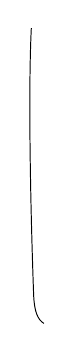
\begin{tikzpicture}[x=1cm,y=1cm]\draw[line width=.35pt] (0,0) .. controls (-.04,-.8) and (-.01,-2.3) .. (.03,-3.4) .. controls (.04,-3.6) and (.08,-3.7) .. (.16,-3.75);\end{tikzpicture}}}
Soi\deleted{\unsure{ent}}\inserted{\unsure{nt|ent}} $E,F,\unsure{C|G}$ trois espaces de Hilbert, soit $u$ une application linéaire \deleted{continue}\inserted{cpt} de $E$ dans $F$, \deleted{$E$} $v$ une application linéaire \deleted{continue}\inserted{cpt} de $F$ dans $\unsure{C|G}$, \deleted{soit $\unsure{u|n}$ un entier positif} enfin soit $f(s_1,\mathord{-}s_n)$ une fonction continue \inserted{symétrique et croissante} de $n$ arguments $s_i\geq0$, telle que \deleted{la fonction} $f(e^{t_1},\mathord{-},e^{t_n})$ soit fonction convexe de $(t_i)\in R^n$. Alors on a

\[
\begin{array}{@{}l@{\qquad}l@{}}
(29)&\displaystyle f(\rho_1(uv),\mathord{-}\rho_n(uv))\leq f(\rho_1(u)\rho_1(v),\mathord{\cdot}\,\mathord{-},\rho_n(u)\rho_n(v)\unsure{,})
\end{array}
\]

En effet, il suffit de \deleted{conjuguer}\inserted{\unsure{l'appliquer|appliquer}} le \deleted{lemme}\inserted{th. 1} \deleted{fondamental, \unsure{corollaire} 1, \unsure{condition}} aux deux suites $(\rho_i(uv))_{i\leq n}$ et $(\rho_i(u)\rho_i(v))_{i=n}$. Les conditions \inserted{a l'hyp. b n° 2°) du th 1.} du \deleted{corollaire 1 de ce lemme} sont satisfaites, \deleted{\unsure{en ef}} en vertu du N° \unsure{?|7}, prop. 2, corollaire 3. \deleted{(\unsure{en effet} \illegible{1})}.

\uline{Corollaire 1} Soient $u$ et $v$ \deleted{comme} dans le th. 3, soit $f(r)$ une fonction continue croissante de $r\geq0$ telle que $f(e^t)$ soit fonction convexe de $t\in R$. Alors, pour \deleted{tout \unsure{nbre}} entier $n>0$, on a

{\reversemarginpar\margin{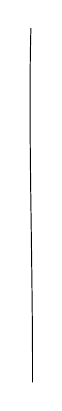
\begin{tikzpicture}[x=1cm,y=1cm]\draw[line width=.35pt] (0,0) .. controls (-.035,-1.25) and (.025,-3) .. (.02,-4.5);\end{tikzpicture}}}
{\reversemarginpar\margin{\illegible{1} $\unsure{l}$\\\deleted{\illegible{1}}\\\deleted{\illegible{1}}\\\deleted{\illegible{1}}}}
\[
\begin{array}{@{}l@{\qquad}l@{}}
(30)&\displaystyle \sum_{i=1}^n f(\rho_i(uv))\leq\sum_{i=1}^n f(\rho_i(u)\rho_i(v))
\end{array}
\]

\deleted{d'où} \inserted{d'où}

\[
\begin{array}{@{}l@{\qquad}l@{}}
(3\unsure{1|4})&\displaystyle \sum_{\unsure{j|i}} f(\rho_i(uv))\leq\sum_{i\unsure{\mathord{-}|=}} f(\rho_i(u)\rho_i(v))
\end{array}
\]

(les sommes étant étendues à tous les indices $i$.)

\deleted{\illegible{1} $\unsure{(\rho_i(uv))|(\rho_i(vu))}$ \unsure{associée} \illegible{2} \unsure{des suites} $(\rho_i(u))$}

\deleted{$(\rho_i(v))$ associée à $u$ resp. $v$, \unsure{les|la} $=$s \unsure{majoration|majorations} \deleted{\unsure{pour tout}} que celle qui vaudrait si on avait $\unsure{\cdot}uv)=\rho_i(u)\rho_i(v)$, donc si $u$ et $v$ étaient des \unsure{p}érateurs de multiplication dans $l^{\unsure{?|2}}$ par les \unsure{tes} $(\rho_i(u))$ resp.\textsuperscript{t} $(\rho_i(v))$. \deleted{\unsure{En particularisant}} \inserted{\uline{Mais} \unsure{prévoir|pourquoi|pourrait} aussi.} \deleted{\unsure{ce dernier, il}} donner un corollaire \deleted{qui} analogue \deleted{\uline{\unsure{Théorème 4}} \unsure{Soient}} au corollaire 4 du th. 1, mais \unsure{en|on} laissons \unsure{l'énoncé} \unsure{au} lecteur.}

\deleted{Dans l'inégalité (39), \unsure{prenons} $p$ \unsure{fixé|fini} et \unsure{très} \illegible{1} $q$ vers $0$, \unsure{d'où|$u$} donné par (30) \illegible{1} et \unsure{on obtient} à la \unsure{limit}}

{\reversemarginpar\margin{92}}
